\begin{activity}\label{A:0.6.2}
	For each of the following graphs, find a possible formula for the polynomial of lowest degree that fits the graph.
    \def\scl{0.7}
				\begin{center}
                    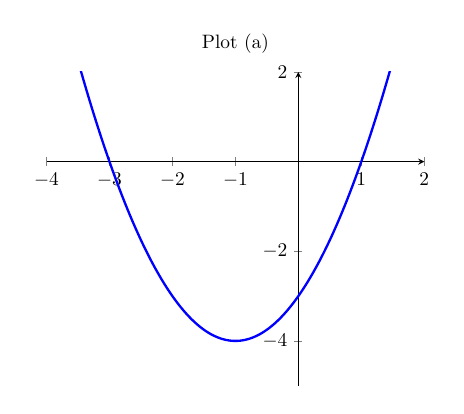
\begin{tikzpicture}[scale=\scl]
                        \begin{axis}[axis lines=center, xmin=-4, xmax=2, ymin=-5, ymax=2,
                            title={Plot (a)}]
                            \addplot[very thick, blue, smooth,samples=100,domain=-4.0:2.0] {((x)-1.0)*((x)+3.0)};
                        \end{axis}
                    \end{tikzpicture}
                    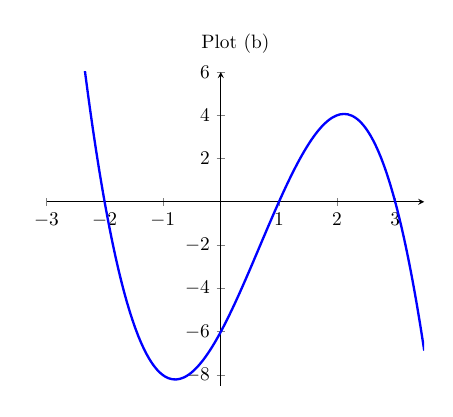
\begin{tikzpicture}[scale=\scl]
                        \begin{axis}[axis lines=center, xmin=-3, xmax=3.5, ymin=-8.5, ymax=6,
                            title={Plot (b)}, ytick={-8,-6,-4,-2,2,4,6}]
                            \addplot[very thick, blue, smooth,samples=100,domain=-3:3.5] {0-((x)+2.0)*((x)-3.0)*((x)-1.0)};
                        \end{axis}
                    \end{tikzpicture}
                    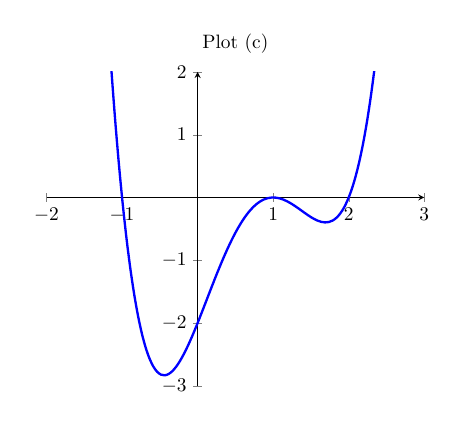
\begin{tikzpicture}[scale=\scl]
                        \begin{axis}[axis lines=center, xmin=-2, xmax=3, ymin=-3, ymax=2,
                            title={Plot (c)}]
                            \addplot[very thick, blue, smooth,samples=100,domain=-2:3] {((x)+1.0)*((x)-2.0)*((x)-1.0)*((x)-1.0)};
                        \end{axis}
                    \end{tikzpicture}
% 					\begin{tikzpicture}[line cap=round,line join=round,>=triangle 45, x=1.0cm, y=0.86cm] 
% 						\draw[->,color=black] (-4.0,0.0) -- (2.0,0.0);
% 						\foreach \x in {-4,-3,-2,-1,1}
% 						\draw[shift={(\x,0)},color=black] (0pt,2pt) -- (0pt,-2pt) node[below] {\footnotesize $\x$};
% 						\draw[->,color=black] (0.0,-5.0) -- (0.0,2.0);
% 						\foreach \y in {-5,-4,-3,-2,-1,1}
% 						\draw[shift={(0,\y)},color=black] (2pt,0pt) -- (-2pt,0pt) node[left] {\footnotesize $\y$};
% 						\draw[color=black] (0pt,-10pt) node[right] {\footnotesize $0$};
% 						\clip(-4.0,-5.0) rectangle (2.0,2.0);
% 						\draw[very thick, blue, smooth,samples=100,domain=-4.0:2.0] plot(\x,{((\x)-1.0)*((\x)+3.0)});
% 					\end{tikzpicture}   
% 					\begin{tikzpicture}[line cap=round,line join=round,>=triangle 45, x=0.86cm, y=0.33cm] 
% 						\draw[<->,color=black] (-3.5,0.0) -- (3.5,0.0); 
% 						\foreach \x in {-3,-2,-1,1,2,3} 
% 						\draw[shift={(\x,0)},color=black] (0pt,2pt) -- (0pt,-2pt) node[below] {\footnotesize $\x$}; 
% 						\draw[->,color=black] (0.0,-10) -- (0.0,8); 
% 						\foreach \y in {-8,-6,-4,-2,2,4,6}
% 						\draw[shift={(0,\y)},color=black] (2pt,0pt) -- (-2pt,0pt) node[left] {\footnotesize $\y$}; 
% 						\draw[color=black] (0pt,-10pt) node[right] {\footnotesize $0$}; 
% 						\clip(-3.5,-10) rectangle (3.5,8); 
% 						\draw[very thick, blue, smooth,samples=100,domain=-3.5:3.5] plot(\x,{0-((\x)+2.0)*((\x)-3.0)*((\x)-1.0)});
% 					\end{tikzpicture}   
% 					\begin{tikzpicture}[line cap=round,line join=round,>=triangle 45, x=1.2cm, y=1.1cm] 
% 						\draw[<->,color=black] (-2,0.0) -- (3,0.0); 
% 						\foreach \x in {-2,-1,1,2,3} 
% 						\draw[shift={(\x,0)},color=black] (0pt,2pt) -- (0pt,-2pt) node[below] {\footnotesize $\x$}; 
% 						\draw[->,color=black] (0.0,-3.5) -- (0.0,2); 
% 						\foreach \y in {-3,-2,-1,1,2}
% 						\draw[shift={(0,\y)},color=black] (2pt,0pt) -- (-2pt,0pt) node[left] {\footnotesize $\y$}; 
% 						\draw[color=black] (0pt,-10pt) node[right] {\footnotesize $0$}; 
% 						\clip(-2,-3.5) rectangle (3,2); 
% 						\draw[very thick, blue, smooth,samples=100,domain=-2:3] plot(\x,{((\x)+1.0)*((\x)-2.0)*((\x)-1.0)*((\x)-1.0)}); 
% 					\end{tikzpicture}   
				\end{center}      
\end{activity}\aftera
